% This is a sample LaTeX input file.  (Version of 9 April 1986) 
% 
% A '%' character causes TeX to ignore all remaining text on the line, 
% and is used for comments like this one.

\documentclass{article}    % Specifies the document style.
\usepackage{graphicx}
\usepackage{alltt}
\title{Ontology Engineering \& Semantic Web \\ Project Report}  % Declares the document's title. 
\author{Panagiotis Chatzichristodoulou and Kirill Tumanov}    % Declares the author's name
\date{March 27, 2014}   % Deleting this command produces today's date.

%
\begin{document}           % End of preamble and beginning of text.
%
\maketitle                 % Produces the title.
%
\begin{abstract}
%
This work serves as a reference and a summary document for the designed Student Lifecycle Management (SLM) system ontology, based on the SAP AG framework. It gives an overall structure of the ontology and describes the main functions of student lifecycle it reflects. For better comprehension this description is coupled with following the built-it exemplar individuals. The paper ends with discussion on ontology limitations and possible future work.
%
\end{abstract}
%
% 
\section{Introduction}
%
Ontology engineering is a field that studies the methods and methodologies of building ontologies. From an Artificial Intelligence point of view, an ontology is defined as: ``explicit specification of conceptualization''~\cite{Gruber}, meaning that ontologies are formal representations of sets of concepts and the relations between them within a domain. It must be noted that even though ontologies are build to serve as formal representations of a certain problem, ontologies should be build as problem-independent as possible. Consequently, an ontology about a car of a certain brand must also be able to represent cars of other brads without any modifications. The domain of the ontology described in this paper is the domain of SLM, meaning that the ontology build creates a framework that describes the Student Lifecycle Management system. Despite the fact that it was based on SAP-SLM~\cite{sap}, the ontology can represent a much wider range of student lifecycle management systems.
\\
For the creation of the ontology Protege tool was used. For the visualization and the analysis of the ontology, protege plugins \textit{OntoGraph}~\cite{protegeOntoGraph} and \textit{CloudView}~\cite{protegeCloudViews} were used. The ontology created abides by the \textit{OntoClean}~\cite{ontoCleanPaper} standards.
% 
\section{Implementation}
%
The ontology of SLM system was designed according to the available SAP AG framework, shown in Fig.~\ref{SAP}.
\begin{figure}[htbp]
  \centering
    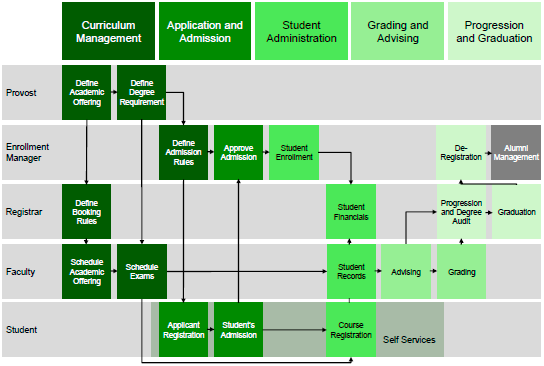
\includegraphics[width=0.8\textwidth]{Materials/Figures/1.png}
    \caption{SAP AG framework of SLM~\cite{sap}}
  \label{SAP}
\end{figure}

Although there is no clear specification of what procedures the system is able to reflect, it is relatively easy to understand what are the most essential ones. Some of the blocks shown here in the ontology were logically merged or united by their roles and underlying processes. E.g. ``Graduation" was merged with ``De-Registration" and has a lot in common with ``Define Degree Requirement". 
A more specific review of the ontology is done in the following subsections. They are organized on the built-in individuals, as a whole student lifecycle process.
%
\subsection{Application and Graduation}
%
Everything started when a British school graduate Bob Smith heard from his friend Joey Miller about the RWTH University, who graduated on the same year. Joey told him that some years ago he was a student at the Mathematics Department of this university. He followed a Study Programme in Mathematics very similar to the one in existence. Upon completion of the studies, he was awarded a BSc Degree in Mathematics, deregistered by Sam Jones - an Enrollment Manager and included into the list of RWTH Alumni. Now Joey was going to attend an Alumni Meeting organized by Terry Mitchel - an Alumni Manager.
Joey inspired Bob to take the same study programme as his, since Bob was quite into Math. So, Bob filed an Admission Request, which includes all needed documents and side procedures, this request was received and fulfilled (processed) by the Enrollment Manager. After the decision was made, the Admission Request resulted in Admission Response, which was sent to Bob. Bob received the Response and found himself accepted to the RWTH. He later was enrolled as a student by the Enrollment Manager. 
% 
\subsection{Study Programme}
%
Bob being a Math student selected to pursue a Study Programme in Mathematics, which culminates with an award of BSc Degree to the graduates. The Study Programme established by a Provost apart from the rest includes courses in Linear Algebra and Statistical Theory. The Programme and all its courses are taught in English. In addition, the Study Programme has a number of specializations, among which are a Major in Mathematics and a Minor in Statistics.
A certain amount of Credits is given for each Course, while it also is awarded to a Student upon a successful completion. A Course in Statistical Theory has a Linear Algebra as a prerequisite. Each Course has an Exam attached; both of them are taught and conducted respectfully by a Faculty. Course as well as Event has a specific location. 


%
% ---- Bibliography ----
%
\begin{thebibliography}{99}
%
\bibitem {sap}
Solution in Detail: Higher Education and Research. Student Life Management.
SAP AG, \texttt{http://www.sap.com/bin/sapcom/en\_us/downloadasset.2013-12-dec\newline-11-11.higher-education-and-research-student-lifecycle-\newline management-pdf.html}(2013)

\bibitem{protege}
Protege ontology creation tool Website.\\
\texttt{http://protege.stanford.edu/}

\bibitem{protegeWiki}
Protege ontology creation tool Wiki.\\
\texttt{http://protegewiki.stanford.edu/wiki/Main\_Page}

\bibitem{protegeCloudViews}
Protege tool cloud views plugin.\\
\texttt{http://protegewiki.stanford.edu/wiki/Cloud\_Views}

\bibitem{protegeOntoGraph}
Protege onto graph views plugin.\\
\texttt{http://protegewiki.stanford.edu/wiki/OntoGraf}

\bibitem{ontoCleanPaper}
Ontoclean Method.\\
\texttt{http://www.researchgate.net/publication/27293101\_Evalu-\newline
ating\_ontological\_decisions\_with\_OntoClean/file/9fcfd50-\newline
f9621161392.pdf}

\bibitem{Gruber}
Gruber T.:
\\
\texttt{http://www-ksl.stanford.edu/kst/ what-is-an-ontology.html.} 



%%%%%%%%%%%%%%%%%%%%%%%%%%%%%%%%%%%%%%%%%%%%%%%%%%%%%%%%%%%%%%%%%%%
\end{thebibliography}
\end{document}             % End of document. 